\chapter{Appendix 3}
\section{Characteristic function and local volume fraction sensitivity distribution}
In this subsection we present the distribution of both characteristic function and local volume fraction sensitivity to the design variables in the example introduced in subsection \ref{SA}. The effect of both the sampling window size and the number of Gauss point is analyzed to compute $\delta$ from the same $W$.
An important observation is that by increasing $N_{GP}$ one increases the ability of GGP to adequately capture the narrow distribution of characteristic function sensitivity.
\begin{figure}[ht]
\centering
\subfloat[$\frac{\partial W}{\partial Y}$]{{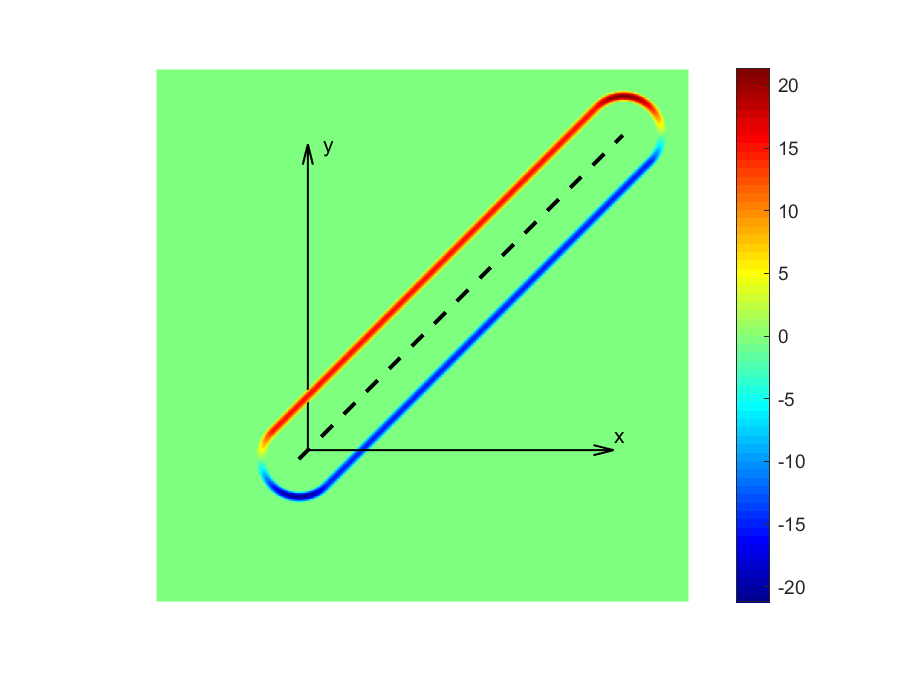
\includegraphics[width=0.4\textwidth]{images/Ch3/dW_dY.eps} }}%
    \subfloat[$\frac{\partial \delta }{\partial Y}$ ,$R=\frac{1}{2}dx$, $N_{gp}=4$]{{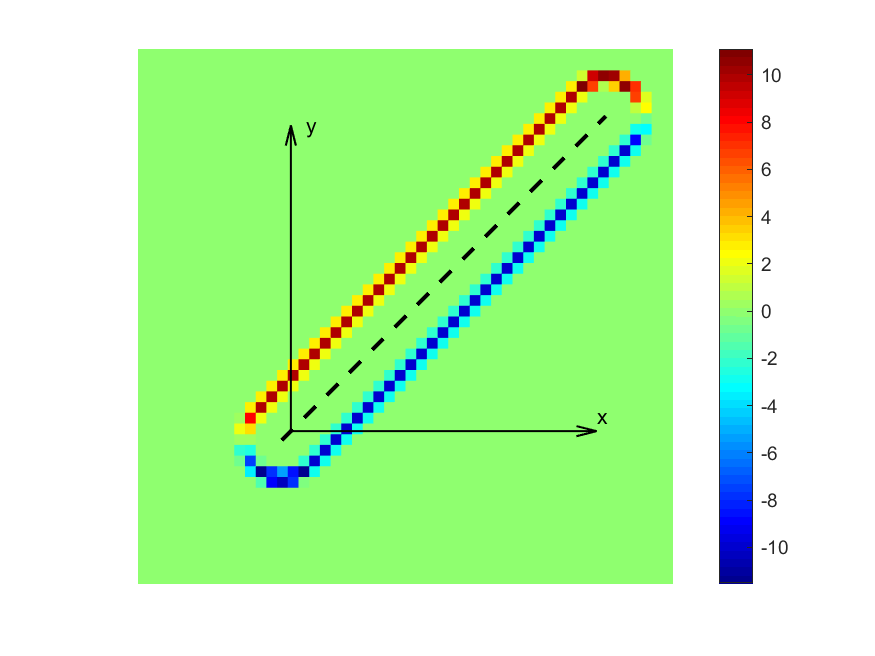
\includegraphics[width=0.4\textwidth]{images/Ch3/ddelta_dY_N_2_R_0_5.png}}}%
     \\
    \subfloat[$\frac{\partial \delta }{\partial Y}$ ,$R=\frac{1}{2}dx$, $N_{gp}=9$]{{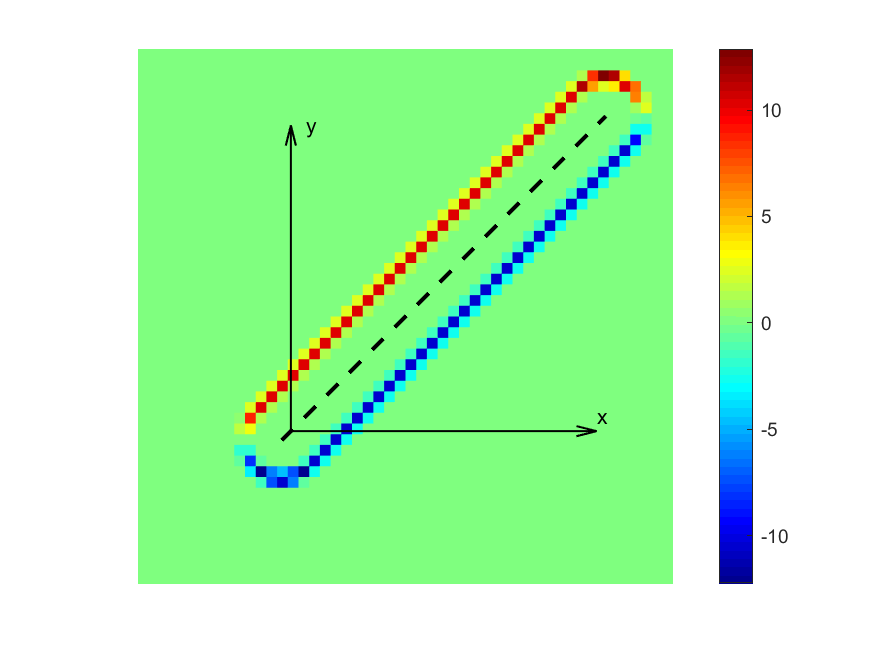
\includegraphics[width=0.4\textwidth]{images/Ch3/ddelta_dY_N_3_R_0_5.png}}}%
    \subfloat[$\frac{\partial \delta }{\partial Y}$ ,$R=dx$, $N_{gp}=4$]{{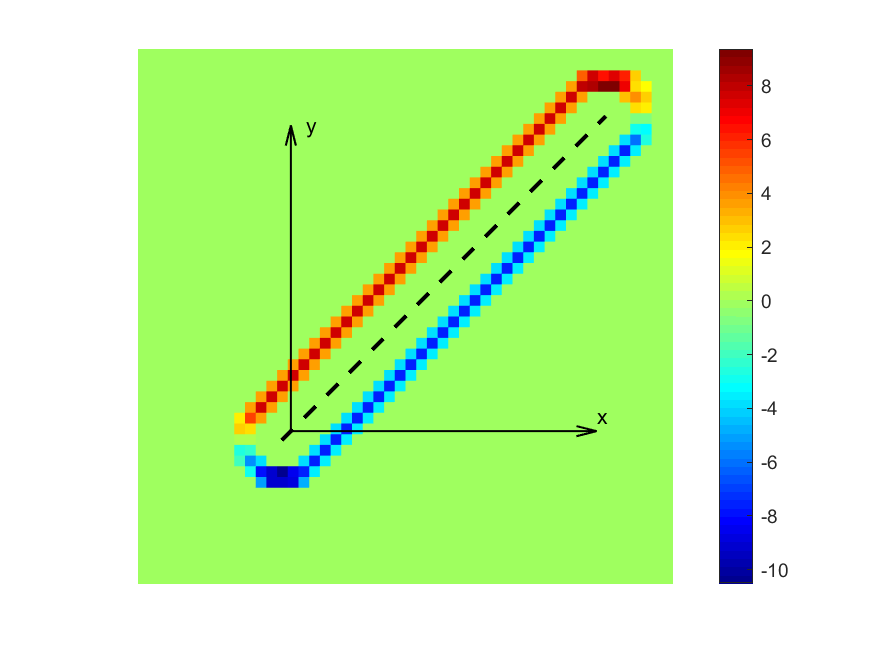
\includegraphics[width=0.4\textwidth]{images/Ch3/ddelta_dY_N_2_R_1.png}}}%
    \caption{Sensitivity distribution of $W$ and $\delta$ with respect to $Y$ for varying number of Gauss Points $N_{GP}$ in the sampling window and varying sampling window size $R$. We considered Adapted Moving Node Approach with the generic component of figure \ref{fig:sc} in the configuration  $X=1,Y=1,L=3,h=0.5,\theta=\frac{\pi}{4}, \gamma=3, \varepsilon=0.07$ and  $dx=0.07$ for a $50\times50$ mesh over the domain of $X_g$.}%
    \label{fig:sensY}%
\end{figure}
\begin{figure}[ht]
\centering
\subfloat[$\frac{\partial W}{\partial L}$]{{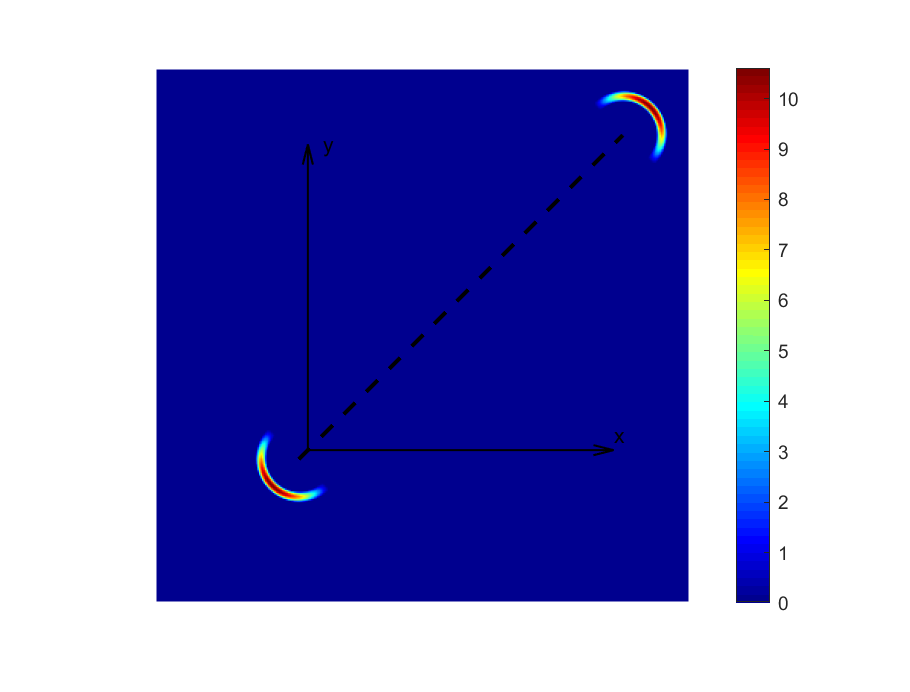
\includegraphics[width=0.4\textwidth]{images/Ch3/dW_dL.eps} }}%
    \subfloat[$\frac{\partial \delta }{\partial L}$ ,$R=\frac{1}{2}dx$, $N_{gp}=4$]{{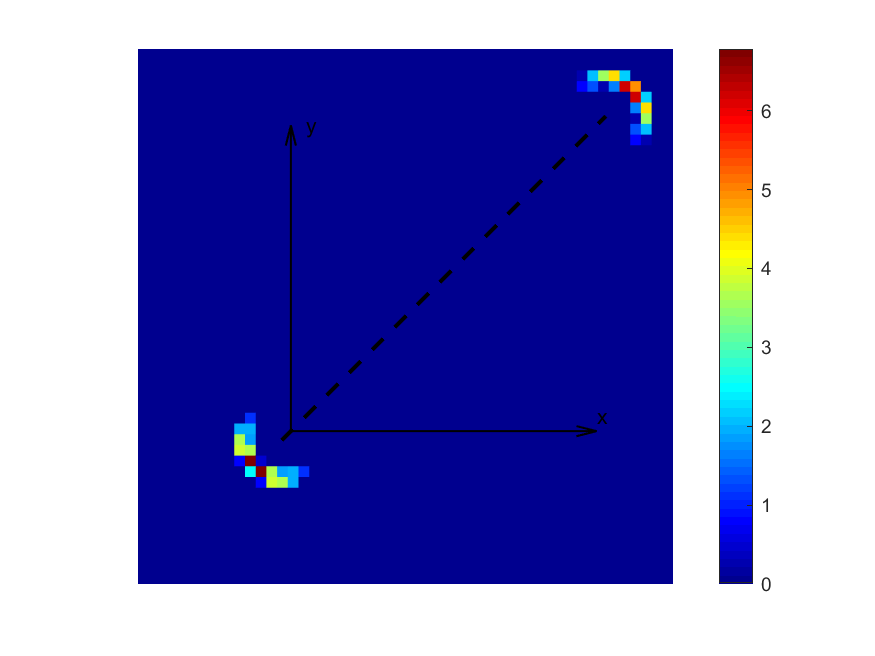
\includegraphics[width=0.4\textwidth]{images/Ch3/ddelta_dL_N_2_R_0_5.png}}}%
     \\
    \subfloat[$\frac{\partial \delta }{\partial L}$ ,$R=\frac{1}{2}dx$, $N_{gp}=9$]{{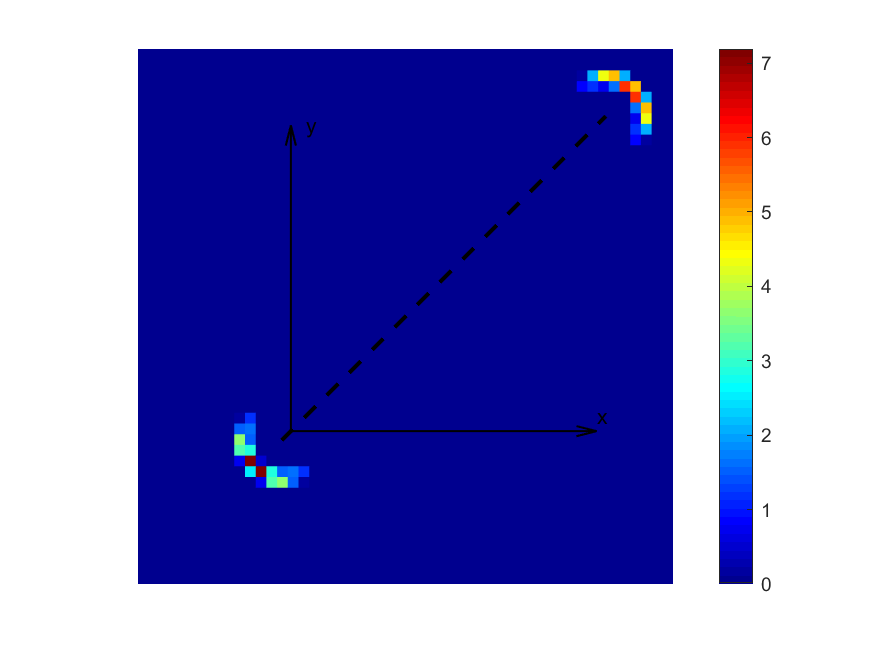
\includegraphics[width=0.4\textwidth]{images/Ch3/ddelta_dL_N_3_R_0_5.png}}}%
    \subfloat[$\frac{\partial \delta }{\partial L}$ ,$R=dx$, $N_{gp}=4$]{{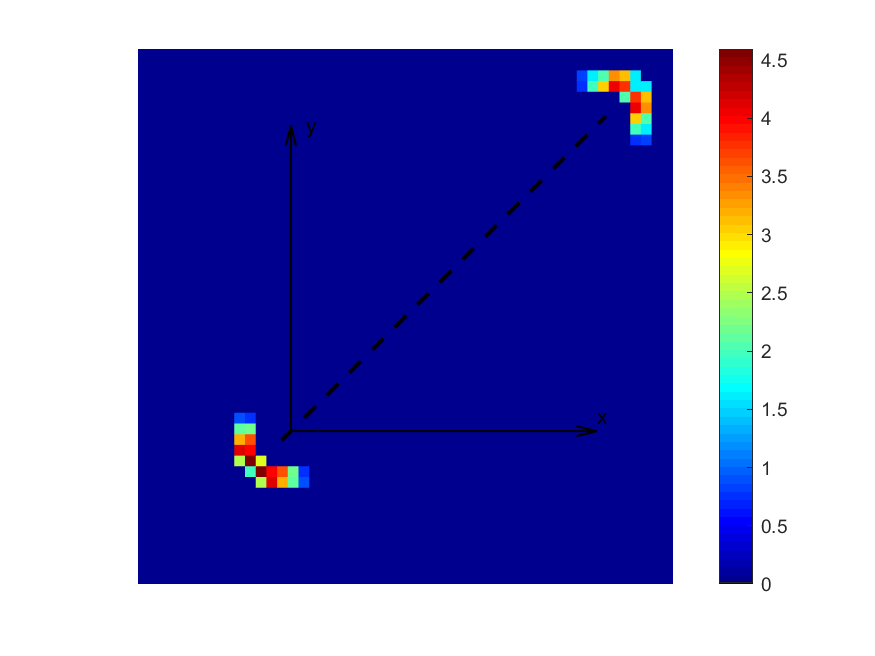
\includegraphics[width=0.4\textwidth]{images/Ch3/ddelta_dL_N_2_R_1.png}}}%
    \caption{Sensitivity distribution of $W$ and $\delta$ with respect to $L$ for varying number of Gauss Points $N_{GP}$ in the sampling window and varying sampling window size $R$. We considered Adapted Moving Node Approach with the generic component of figure \ref{fig:sc} in the configuration  $X=1,Y=1,L=3,h=0.5,\theta=\frac{\pi}{4}, \gamma=3, \varepsilon=0.07$ and  $dx=0.07$ for a $50\times50$ mesh over the domain of $X_g$.}%
    \label{fig:sensL}%
\end{figure}
\begin{figure}[ht]
\centering
\subfloat[$\frac{\partial W}{\partial h}$]{{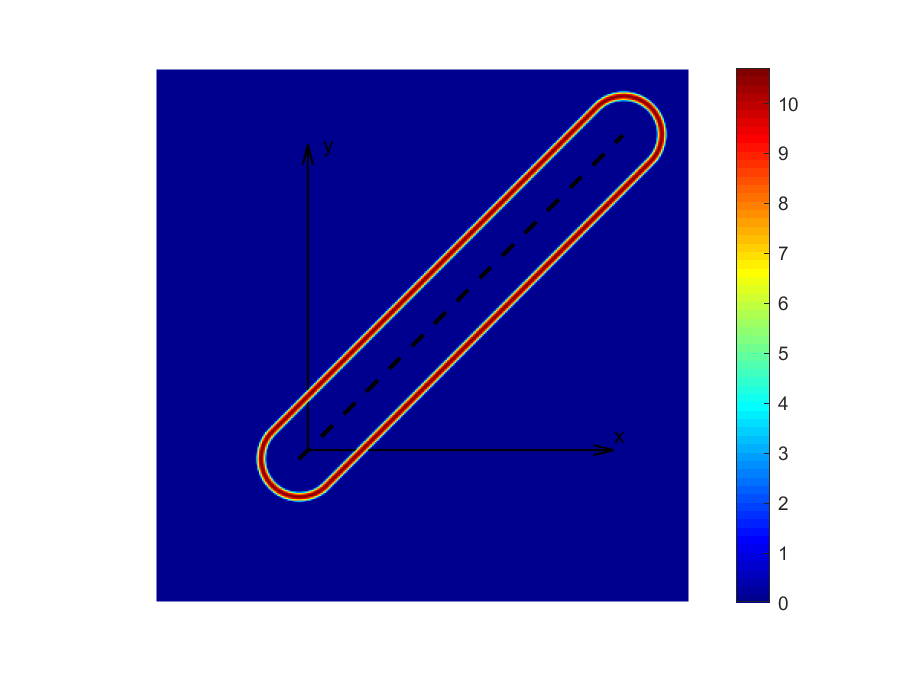
\includegraphics[width=0.4\textwidth]{images/Ch3/dW_dh.eps} }}%
    \subfloat[$\frac{\partial \delta }{\partial h}$ ,$R=\frac{1}{2}dx$, $N_{gp}=4$]{{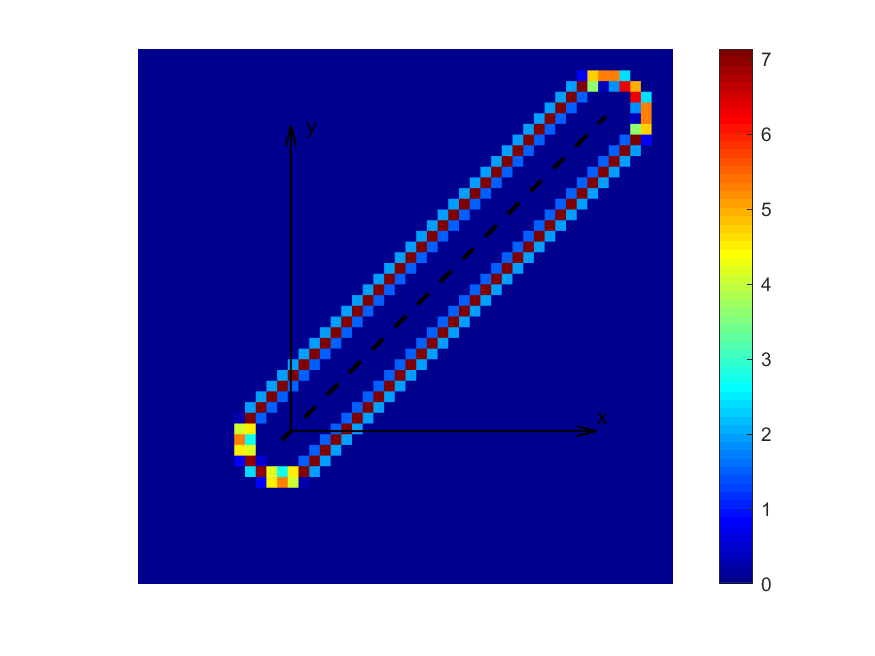
\includegraphics[width=0.4\textwidth]{images/Ch3/ddelta_dh_N_2_R_0_5.png}}}%
    \\
    \subfloat[$\frac{\partial \delta }{\partial h}$ ,$R=\frac{1}{2}dx$, $N_{gp}=9$]{{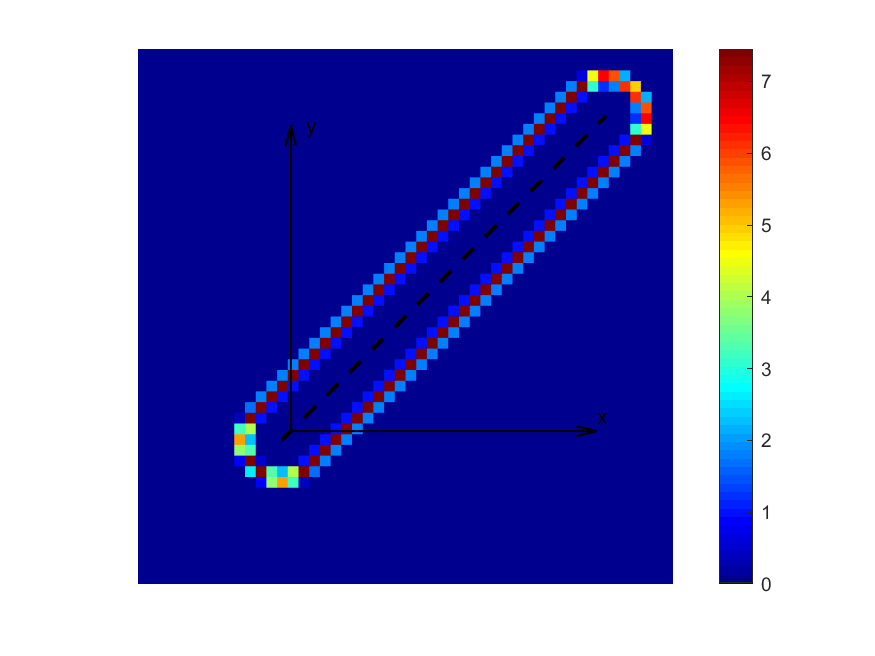
\includegraphics[width=0.4\textwidth]{images/Ch3/ddelta_dh_N_3_R_0_5.png}}}%
    \subfloat[$\frac{\partial \delta }{\partial h}$ ,$R=dx$, $N_{gp}=4$]{{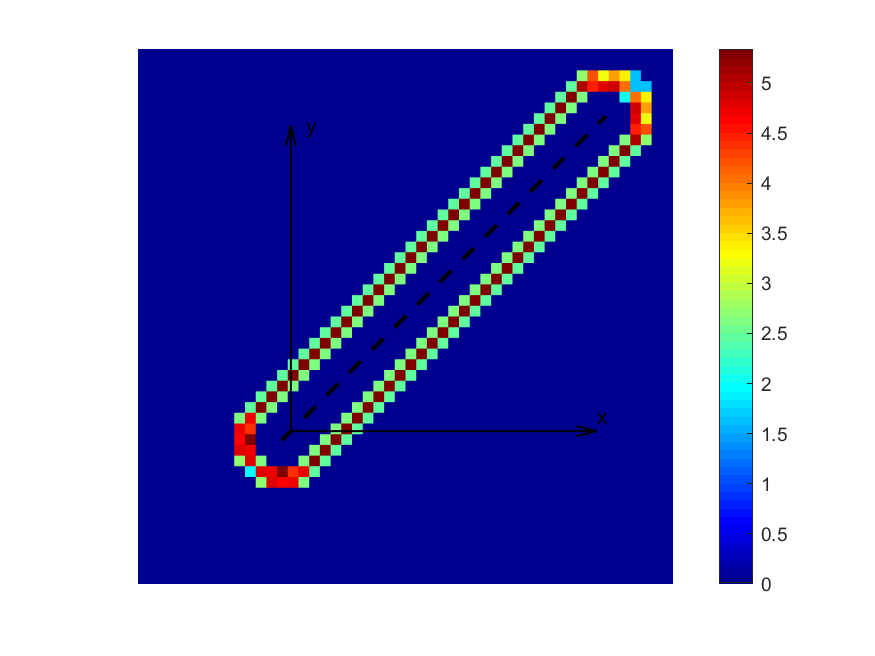
\includegraphics[width=0.4\textwidth]{images/Ch3/ddelta_dh_N_2_R_1.png}}}%
    \caption{Sensitivity distribution of $W$ and $\delta$ with respect to $h$ for varying number of Gauss Points $N_{GP}$ in the sampling window and varying sampling window size $R$. We considered Adapted Moving Node Approach with the generic component of figure \ref{fig:sc} in the configuration  $X=1,Y=1,L=3,h=0.5,\theta=\frac{\pi}{4}, \gamma=3, \varepsilon=0.07$ and  $dx=0.07$ for a $50\times50$ mesh over the domain of $X_g$.}%
    \label{fig:sensh}%
\end{figure}
\begin{figure}[ht]
\centering
\subfloat[$\frac{\partial W}{\partial \theta}$]{{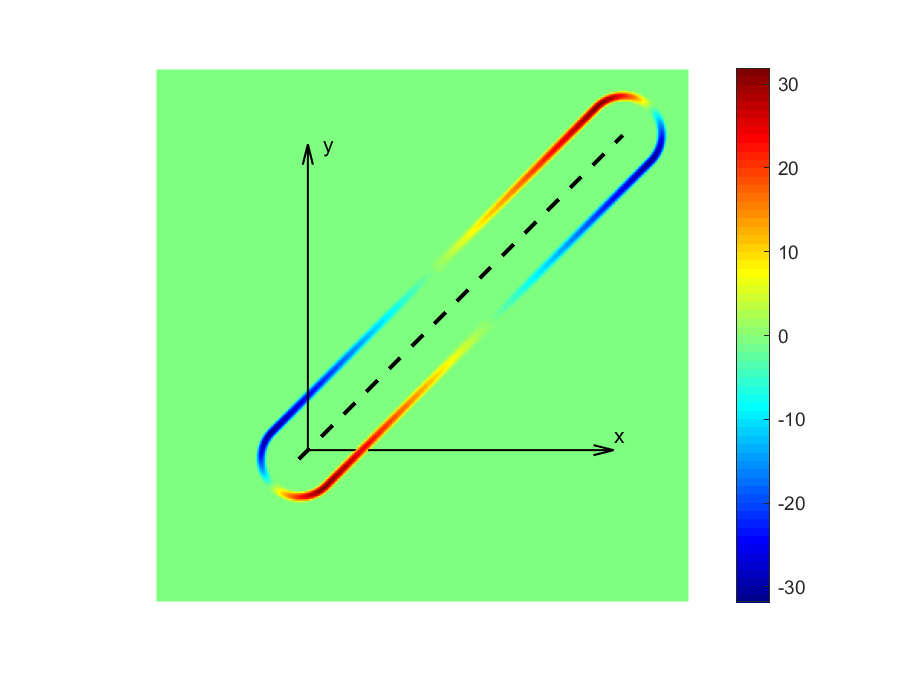
\includegraphics[width=0.4\textwidth]{images/Ch3/dW_dT.eps} }}%
    \subfloat[$\frac{\partial \delta }{\partial \theta}$ ,$R=\frac{1}{2}dx$, $N_{gp}=4$]{{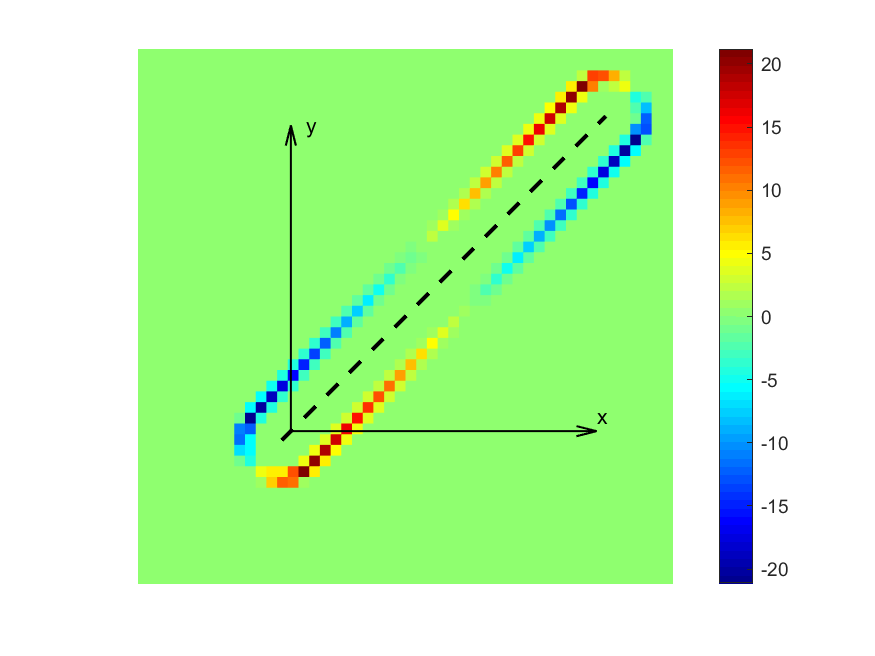
\includegraphics[width=0.4\textwidth]{images/Ch3/ddelta_dT_N_2_R_0_5.png}}}%
     \\
    \subfloat[$\frac{\partial \delta }{\partial \theta}$ ,$R=\frac{1}{2}dx$, $N_{gp}=9$]{{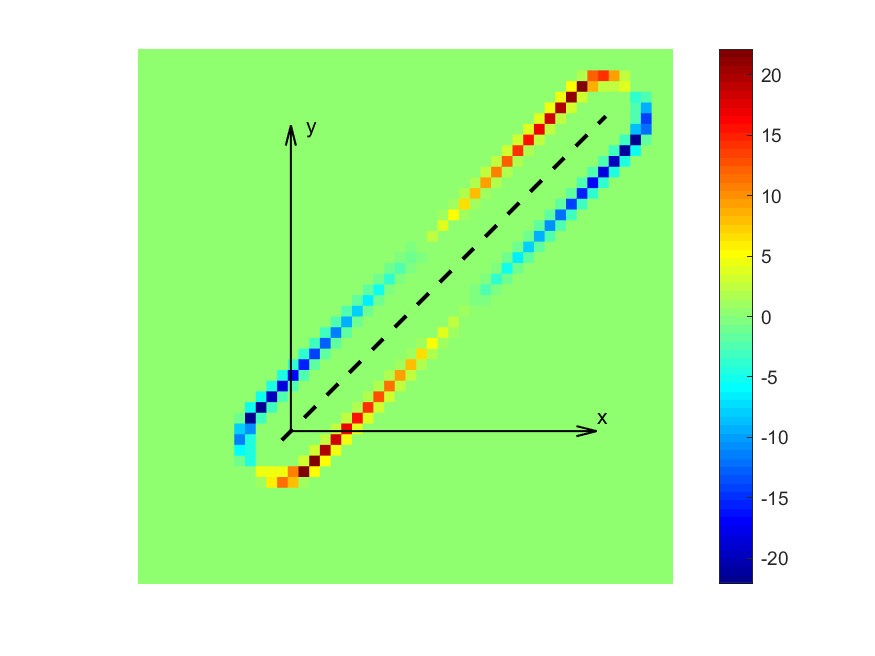
\includegraphics[width=0.4\textwidth]{images/Ch3/ddelta_dT_N_3_R_0_5.png}}}%
    \subfloat[$\frac{\partial \delta }{\partial \theta}$ ,$R=dx$, $N_{gp}=4$]{{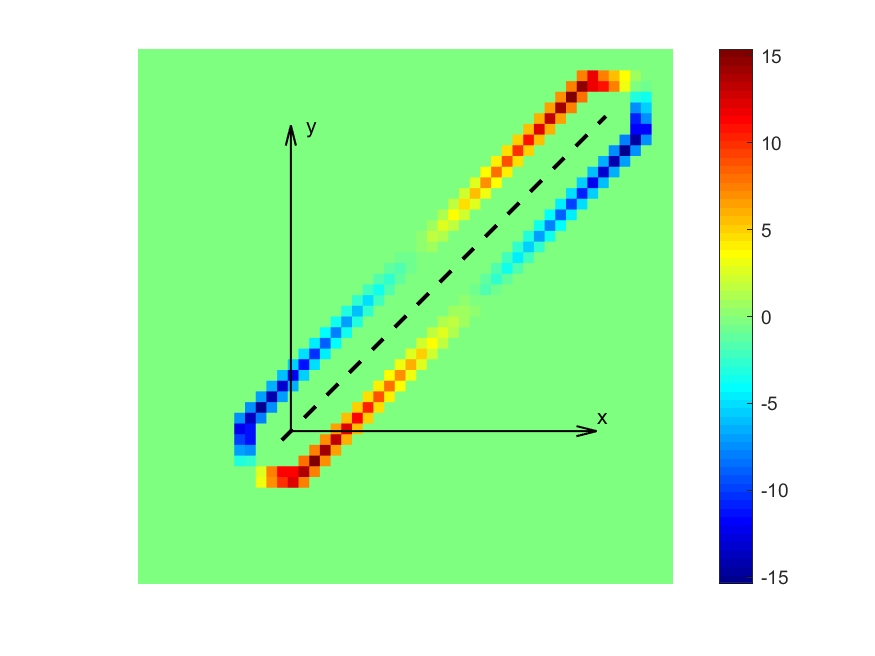
\includegraphics[width=0.4\textwidth]{images/Ch3/ddelta_dT_N_2_R_1.png}}}%
    \caption{Sensitivity distribution of $W$ and $\delta$ with respect to $\theta$ for varying number of Gauss Points $N_{GP}$ in the sampling window and varying sampling window size $R$. We considered Adapted Moving Node Approach with the generic component of figure \ref{fig:sc} in the configuration  $X=1,Y=1,L=3,h=0.5,\theta=\frac{\pi}{4}, \gamma=3, \varepsilon=0.07$ and  $dx=0.07$ for a $50\times50$ mesh over the domain of $X_g$.}%
    \label{fig:sensT}%
\end{figure}

\section{Parametric study results on the cantilever beam case}
In this section the full plot results from the parametric study on the cantilever beam presented in subsection \ref{CB} are provided.
\begin{figure*}
\centering
    \subfloat[$h-C$ plot for $R=\frac{\sqrt{3}}{2}$, $N_{GP}=\vecvar{1,4,16,64}$]{{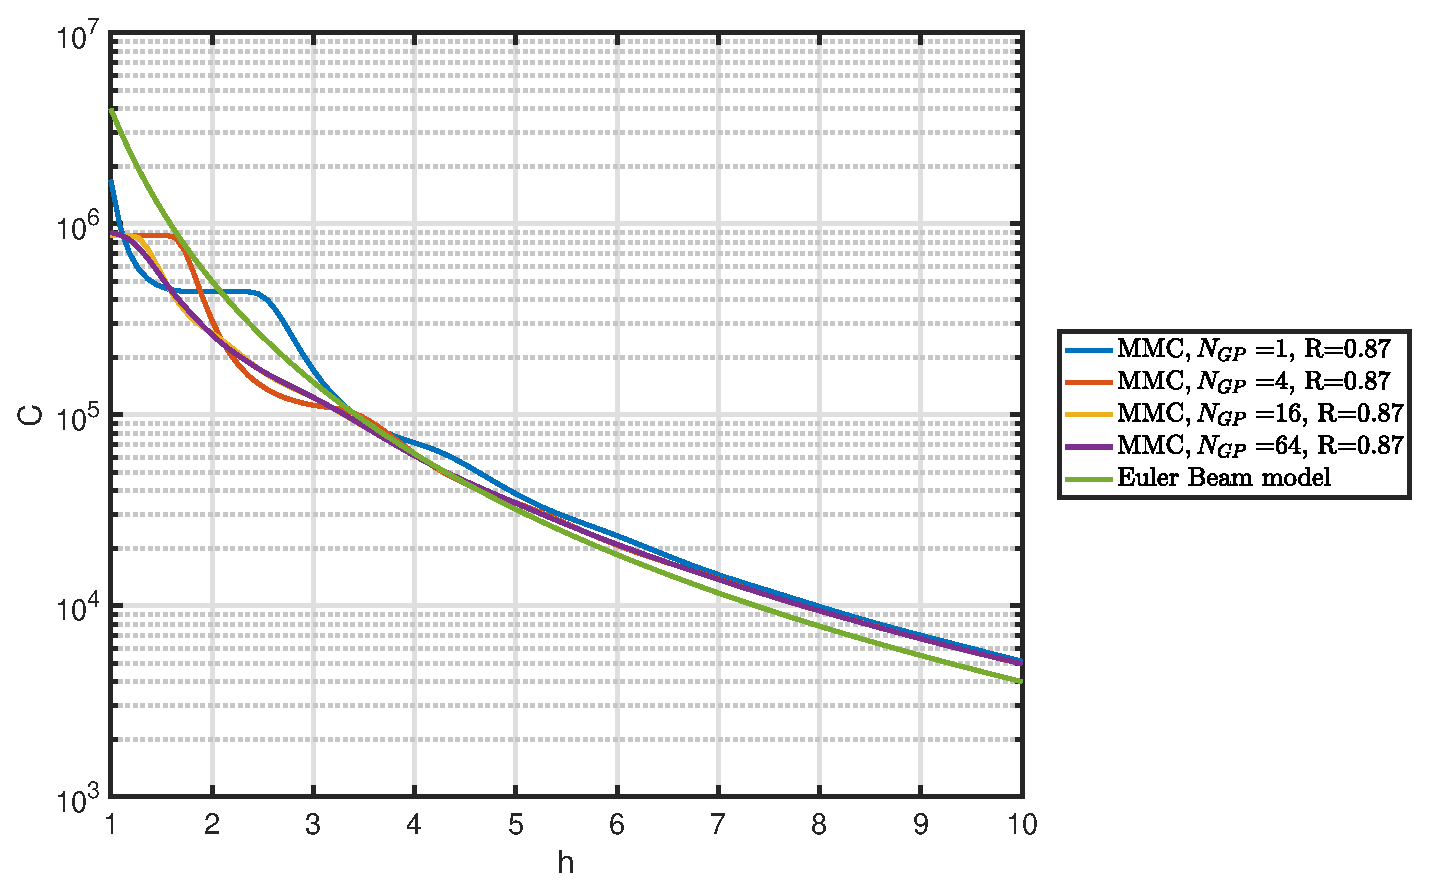
\includegraphics[width=0.4\textwidth]{images/Ch3/31a.eps} }}%
    \quad
    \subfloat[$h-V$ plot for $R=\frac{\sqrt{3}}{2}$, $N_{GP}=\vecvar{1,4,16,64}$]{{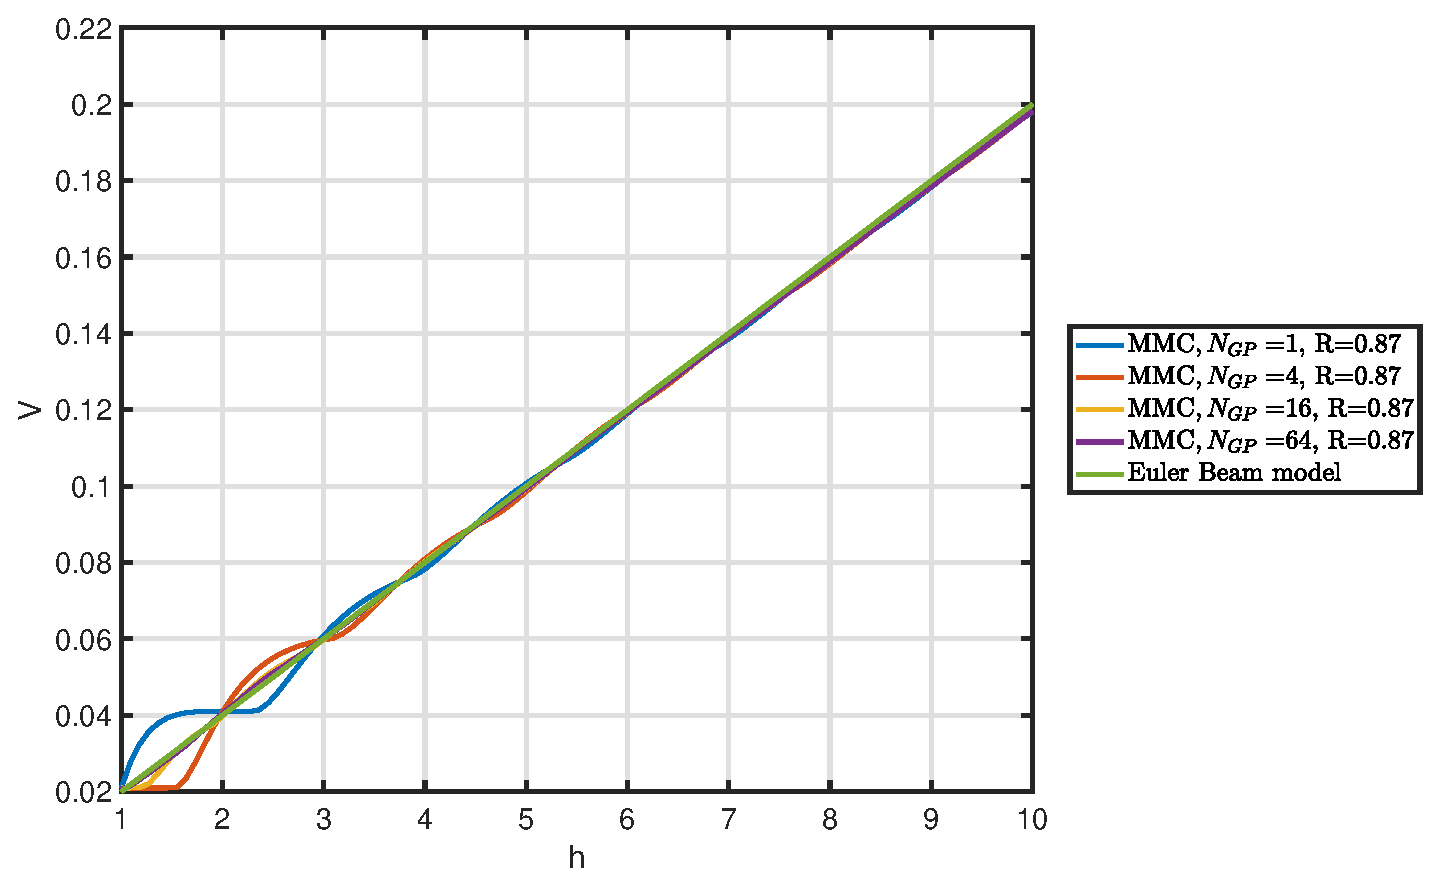
\includegraphics[width=0.4\textwidth]{images/Ch3/31b.eps} }}%
    \\
    \subfloat[$h-C$ plot for $R=1$, $N_{GP}=\vecvar{1,4,16,64}$]{{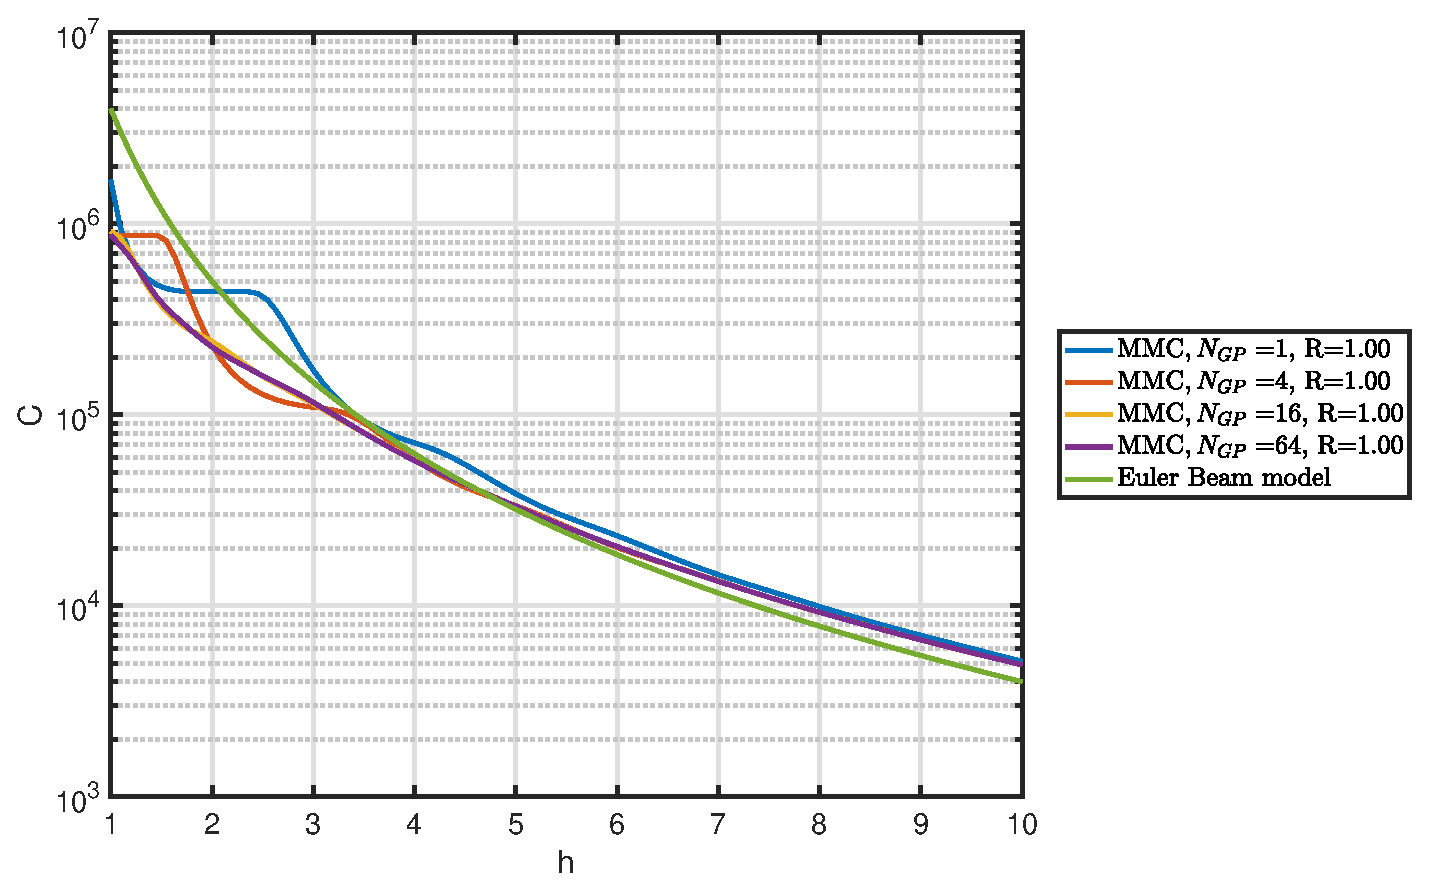
\includegraphics[width=0.4\textwidth]{images/Ch3/31c.eps} }}%
    \quad
    \subfloat[$h-V$ plot for $R=1$, $N_{GP}=\vecvar{1,4,16,64}$]{{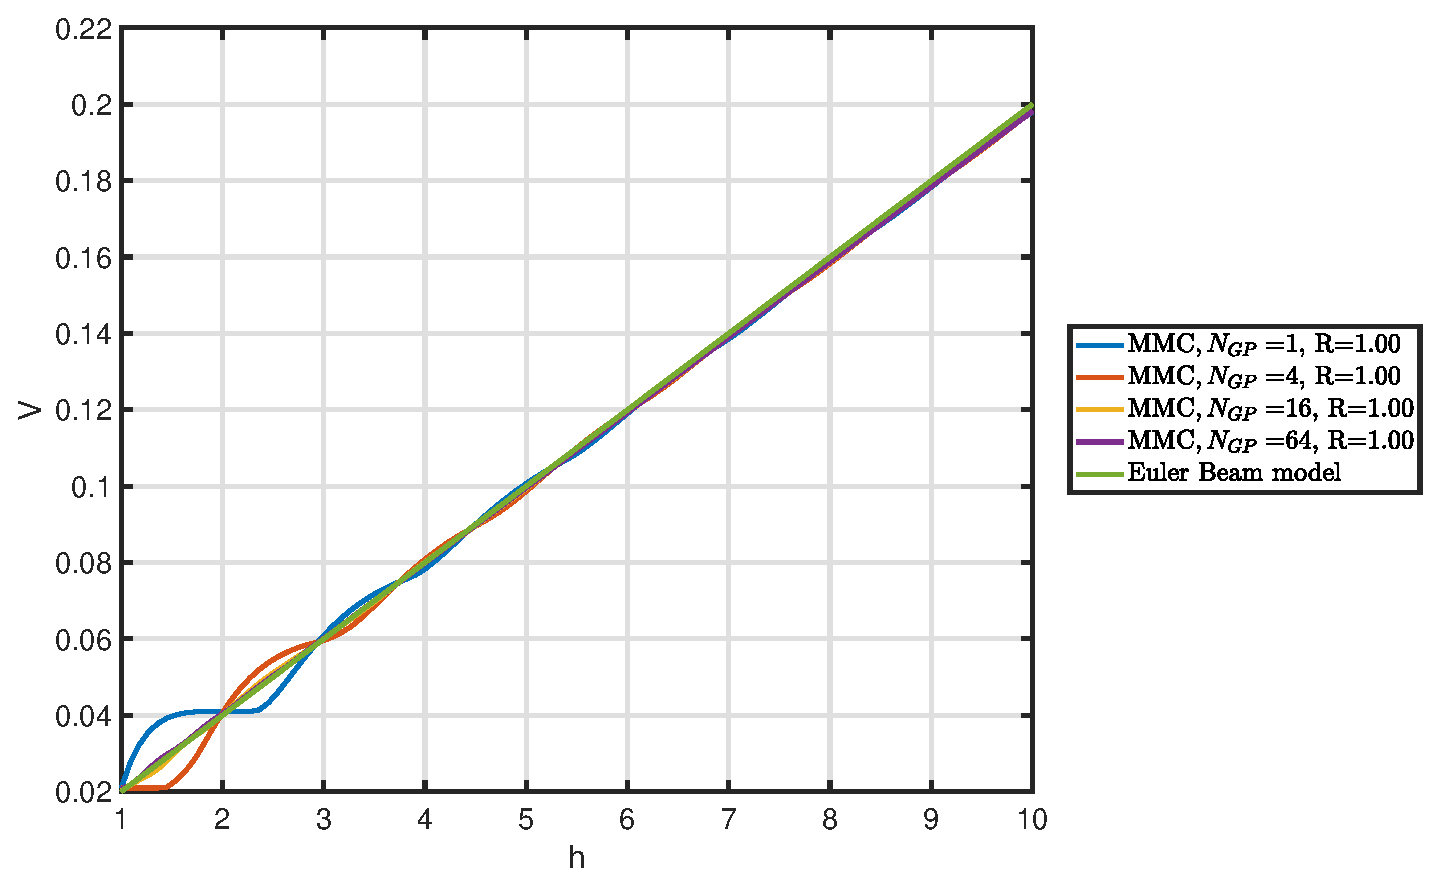
\includegraphics[width=0.4\textwidth]{images/Ch3/31d.eps}}}%
    \caption{Cantilever beam parametric study using the AMMC approach. Effect of the sampling window size $R$ and of the number of Gauss points $N_{GP}$ on the structural compliance and the volume fraction. In each graph we reported in green the true theoretical values based on the analytic beam model.}%
    \label{fig:cbMMC}%
\end{figure*}
\clearpage
\begin{figure*}
\centering
    \subfloat[$h-C$ plot for $R=0.5$, $N_{GP}=\vecvar{1,4,16,64}$]{{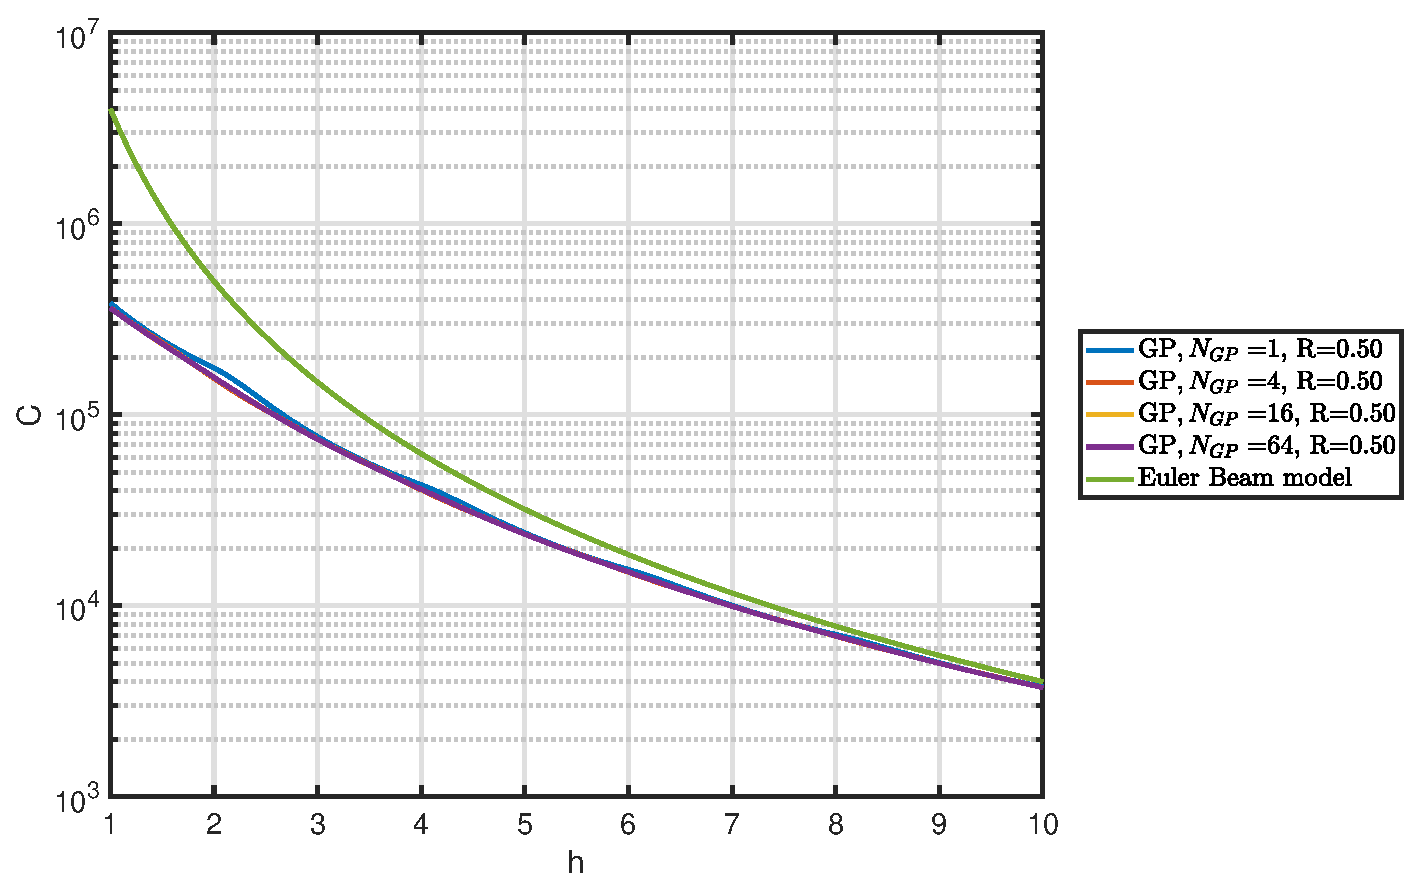
\includegraphics[width=0.4\textwidth]{images/Ch3/32a} }}%
    \quad
    \subfloat[$h-V$ plot for $R=0.5$, $N_{GP}=\vecvar{1,4,16,64}$]{{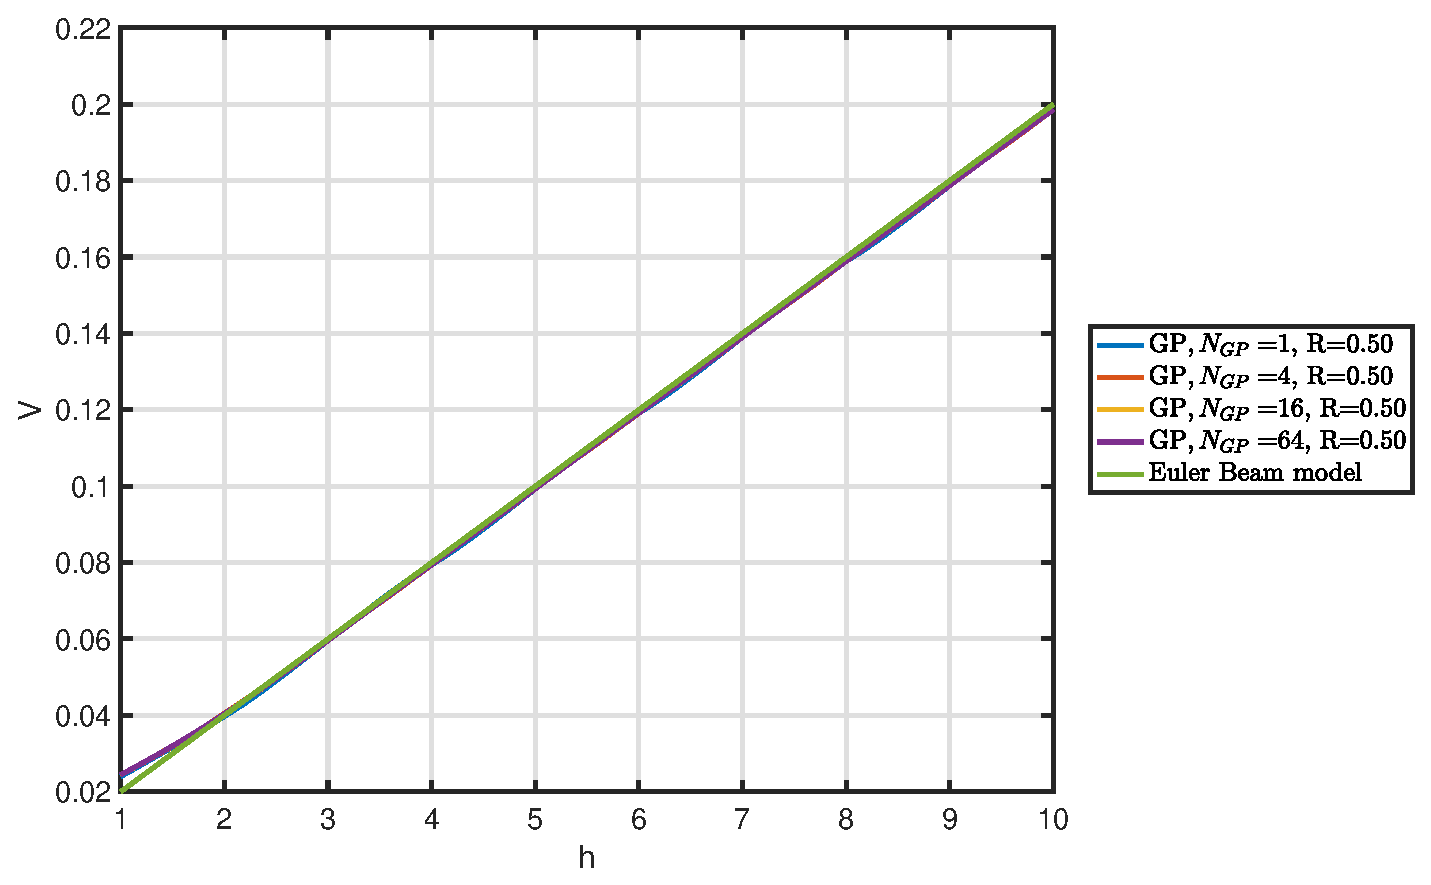
\includegraphics[width=0.4\textwidth]{images/Ch3/32b.eps} }}%
    \\
    \subfloat[$h-C$ plot for $R=\frac{\sqrt{3}}{2}$, $N_{GP}=\vecvar{1,4,16,64}$]{{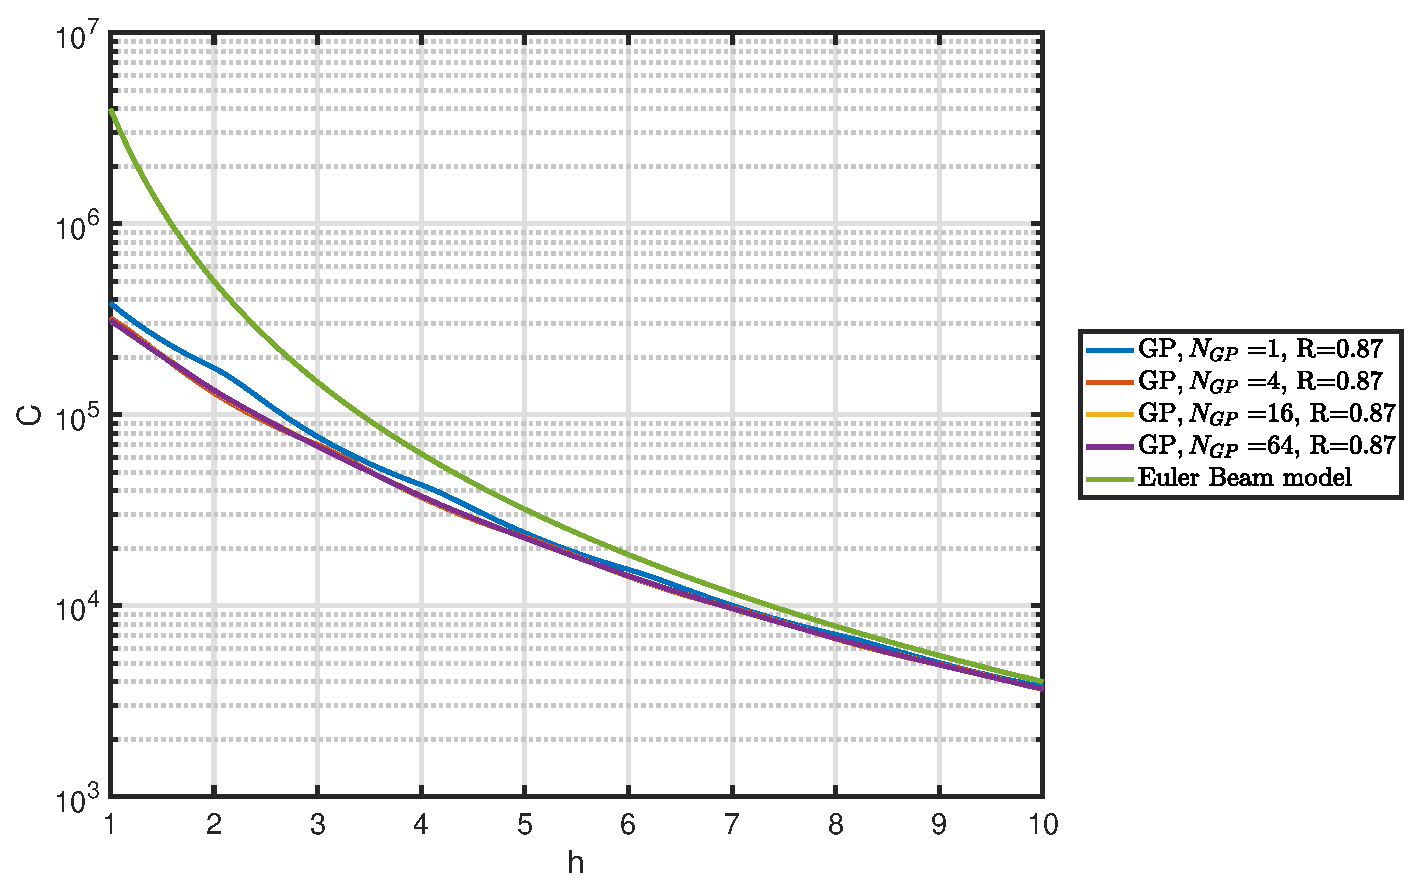
\includegraphics[width=0.4\textwidth]{images/Ch3/32c.eps} }}%
    \quad
    \subfloat[$h-V$ plot for $R=\frac{\sqrt{3}}{2}$, $N_{GP}=\vecvar{1,4,16,64}$]{{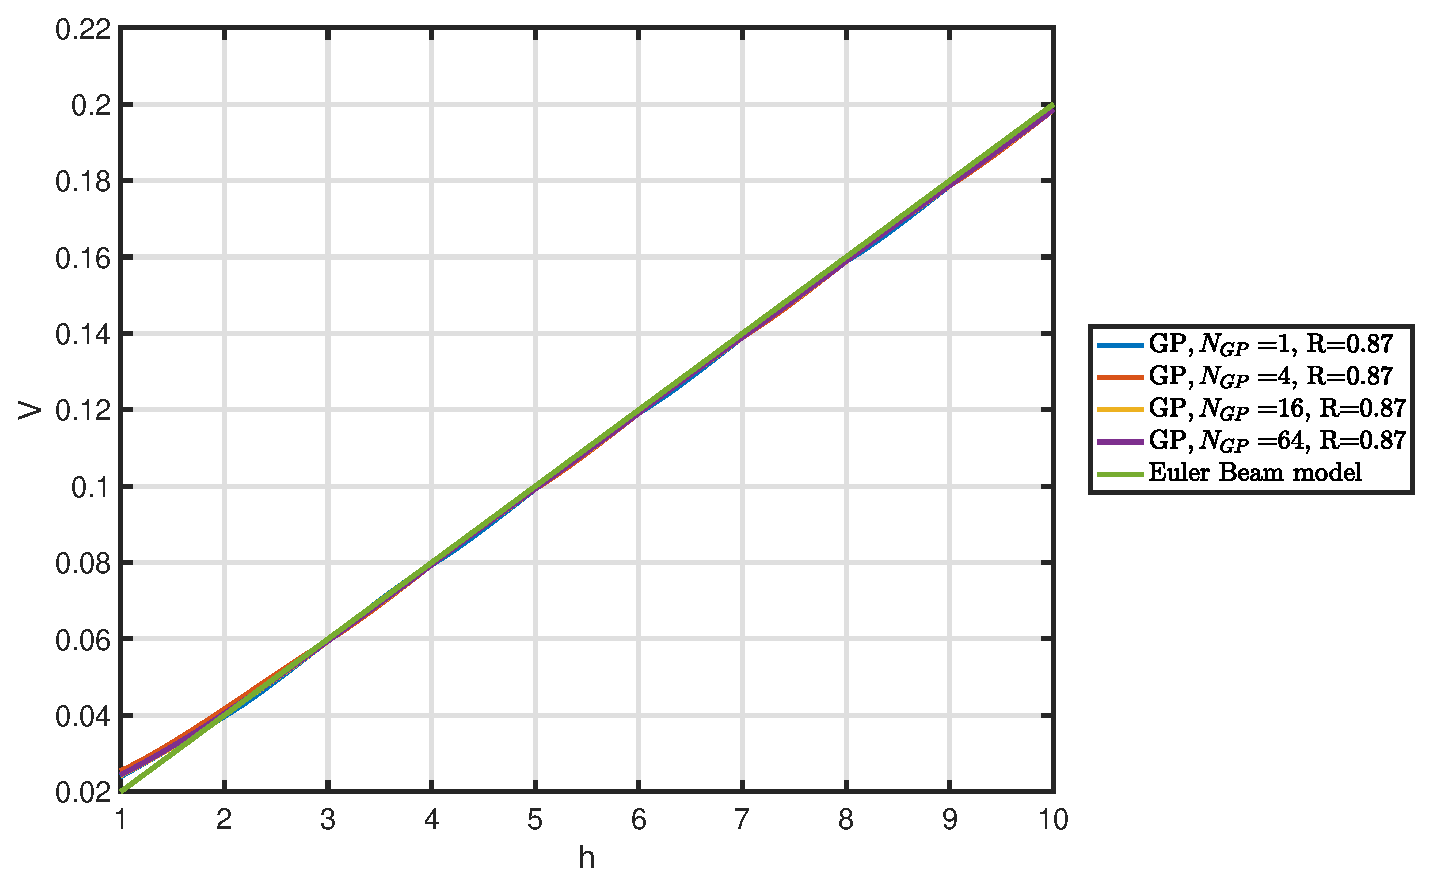
\includegraphics[width=0.4\textwidth]{images/Ch3/32d.eps} }}%
    \\
    \subfloat[$h-C$ plot for $R=1$, $N_{GP}=\vecvar{1,4,16,64}$]{{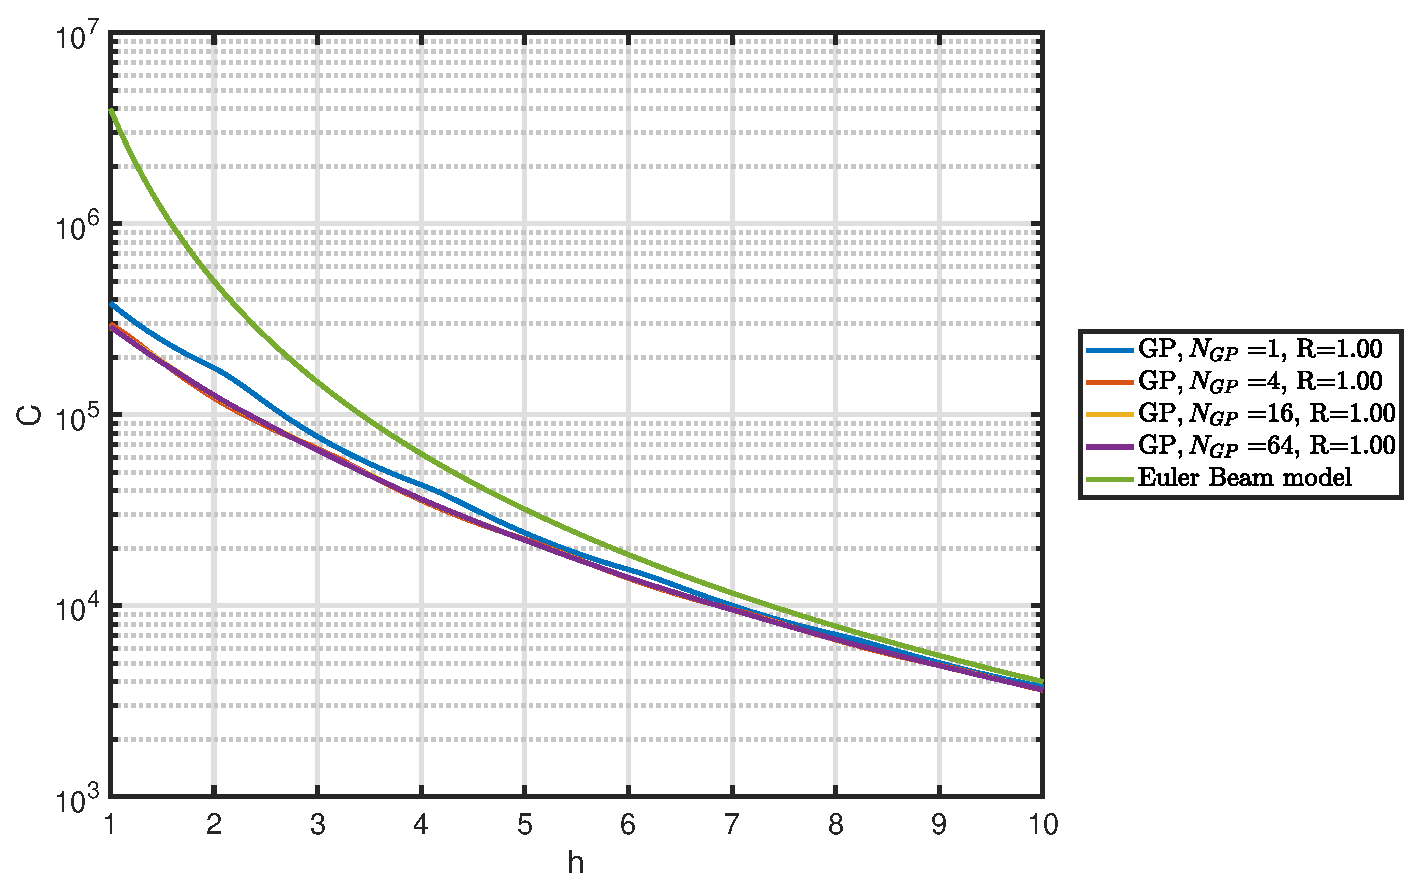
\includegraphics[width=0.4\textwidth]{images/Ch3/32e.eps} }}%
    \quad
    \subfloat[$h-V$ plot for $R=1$, $N_{GP}=\vecvar{1,4,16,64}$]{{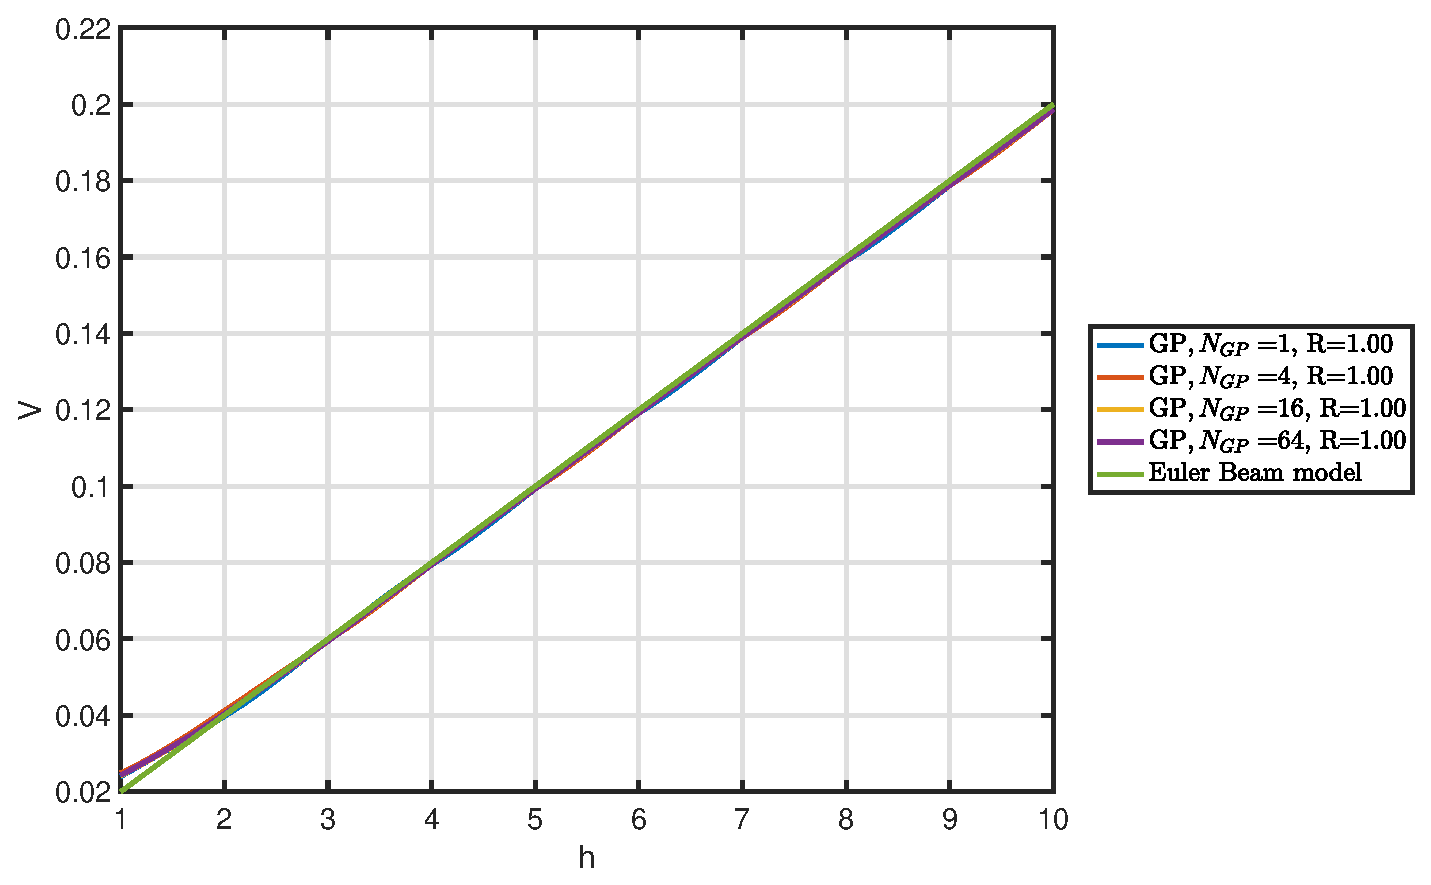
\includegraphics[width=0.4\textwidth]{images/Ch3/32f.eps}}}%
    \caption{Cantilever beam parametric study using AGP method. Effect of the sampling window size $R$ and of the number of Gauss points $N_{GP}$ on the structural compliance and the volume fraction. In each graph we reported in green the true theoretical values based on the analytic beam model.}%
    \label{fig:cbGP}%
\end{figure*}
\begin{figure*}
\centering
    \subfloat[$h-C$ plot for $R=0.5$, $N_{GP}=\vecvar{1,4,16,64}$]{{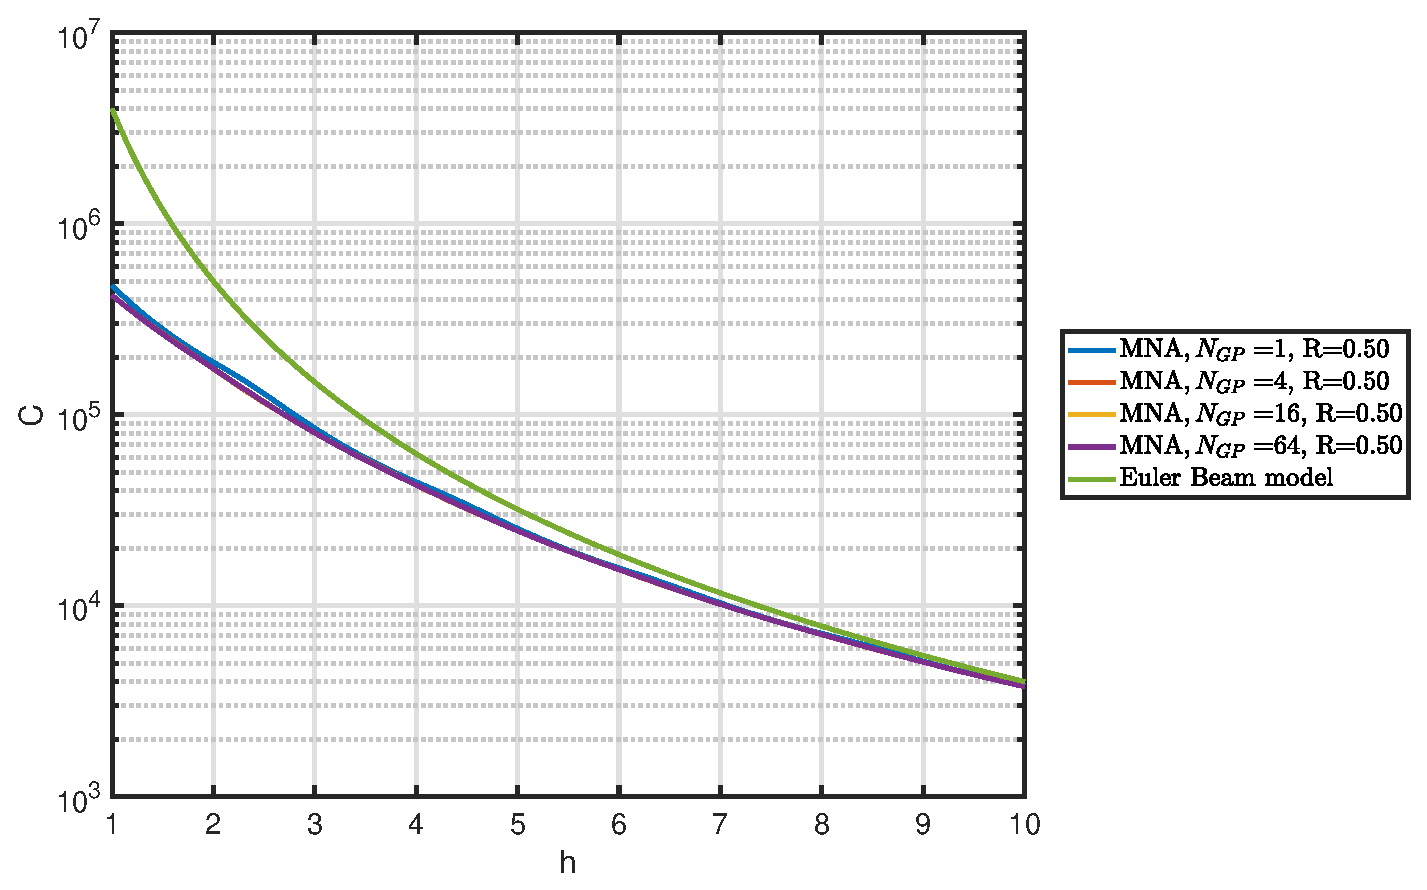
\includegraphics[width=0.4\textwidth]{images/Ch3/33a.eps} }}%
    \quad
    \subfloat[$h-V$ plot for $R=0.5$, $N_{GP}=\vecvar{1,4,16,64}$]{{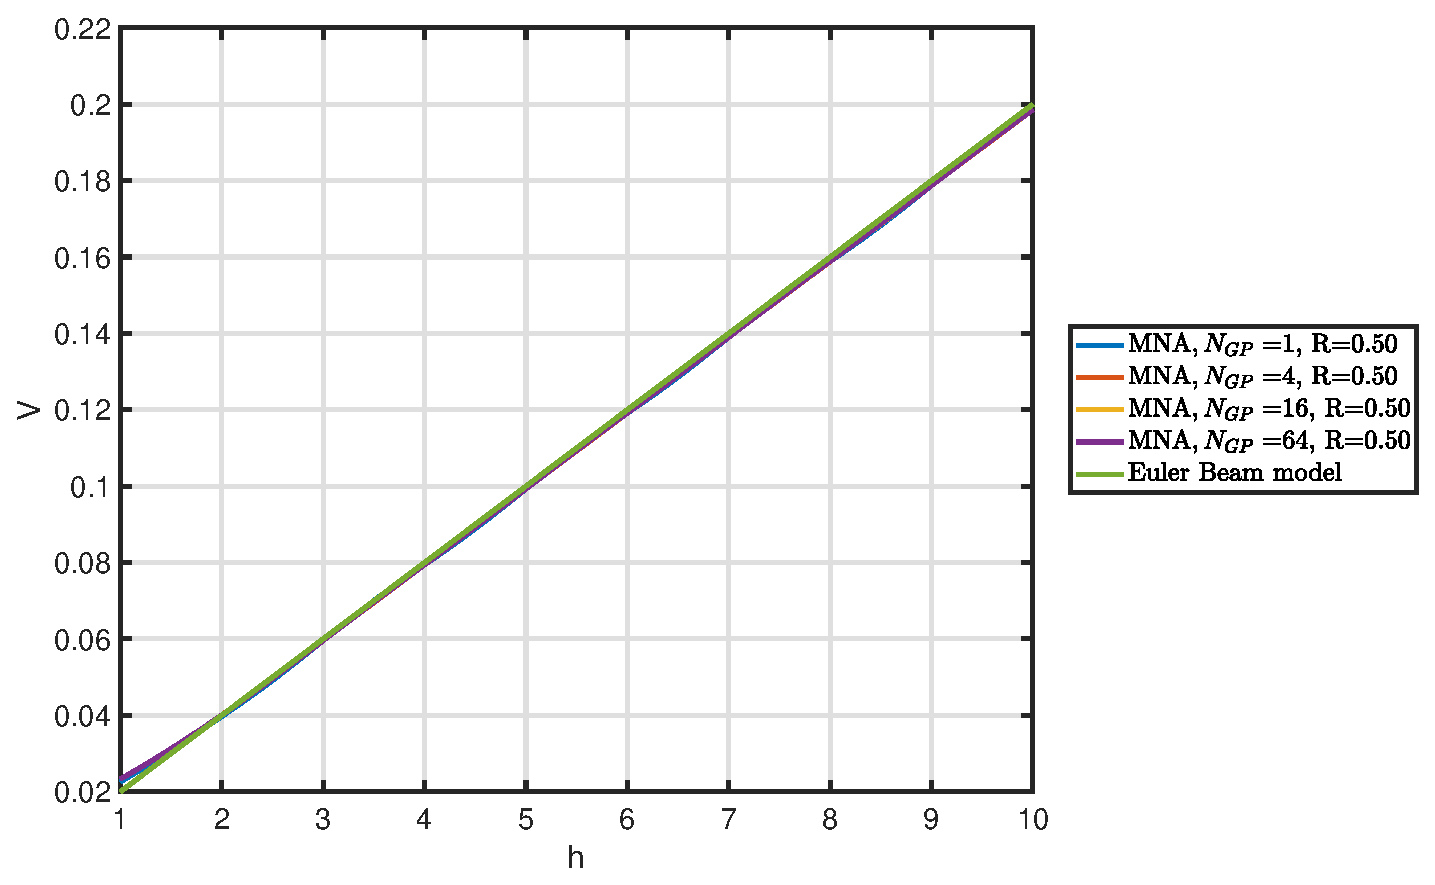
\includegraphics[width=0.4\textwidth]{images/Ch3/33b.eps} }}%
    \\
    \subfloat[$h-C$ plot for $R=\frac{\sqrt{3}}{2}$, $N_{GP}=\vecvar{1,4,16,64}$]{{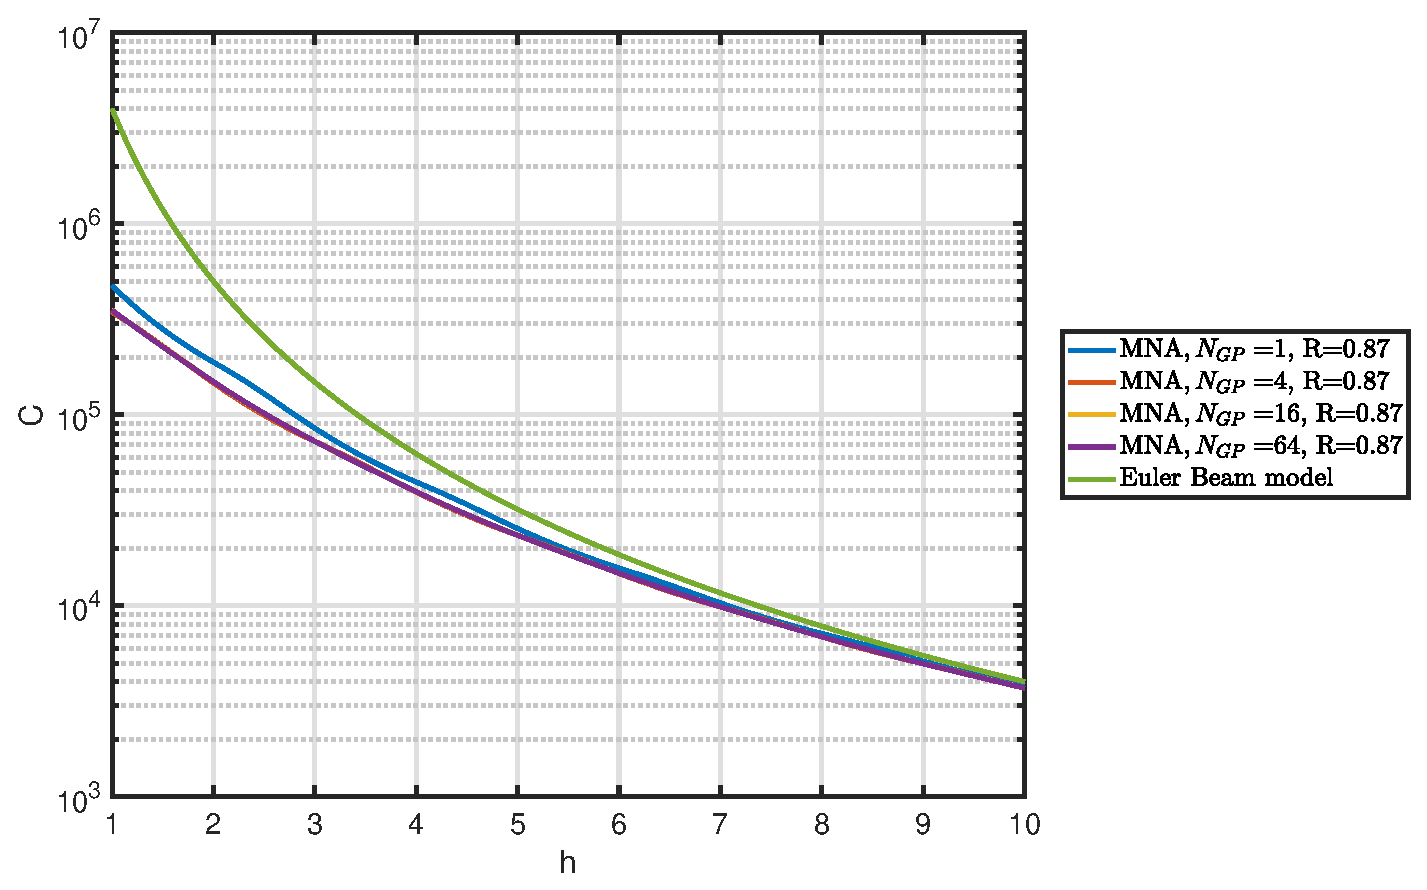
\includegraphics[width=0.4\textwidth]{images/Ch3/33c.eps} }}%
    \quad
    \subfloat[$h-V$ plot for $R=\frac{\sqrt{3}}{2}$, $N_{GP}=\vecvar{1,4,16,64}$]{{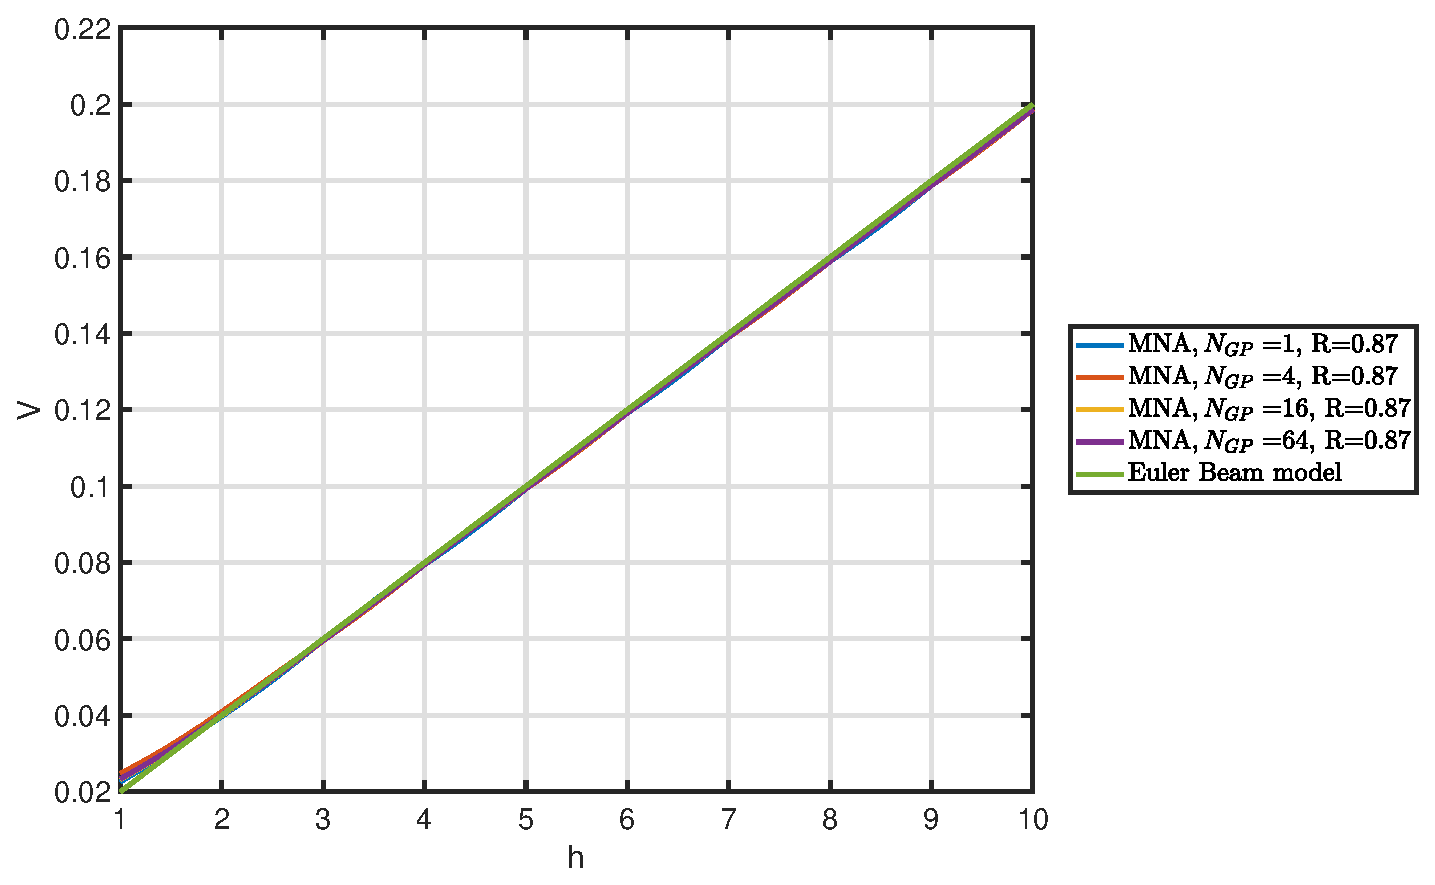
\includegraphics[width=0.4\textwidth]{images/Ch3/33d.eps} }}%
    \\
    \subfloat[$h-C$ plot for $R=1$, $N_{GP}=\vecvar{1,4,16,64}$]{{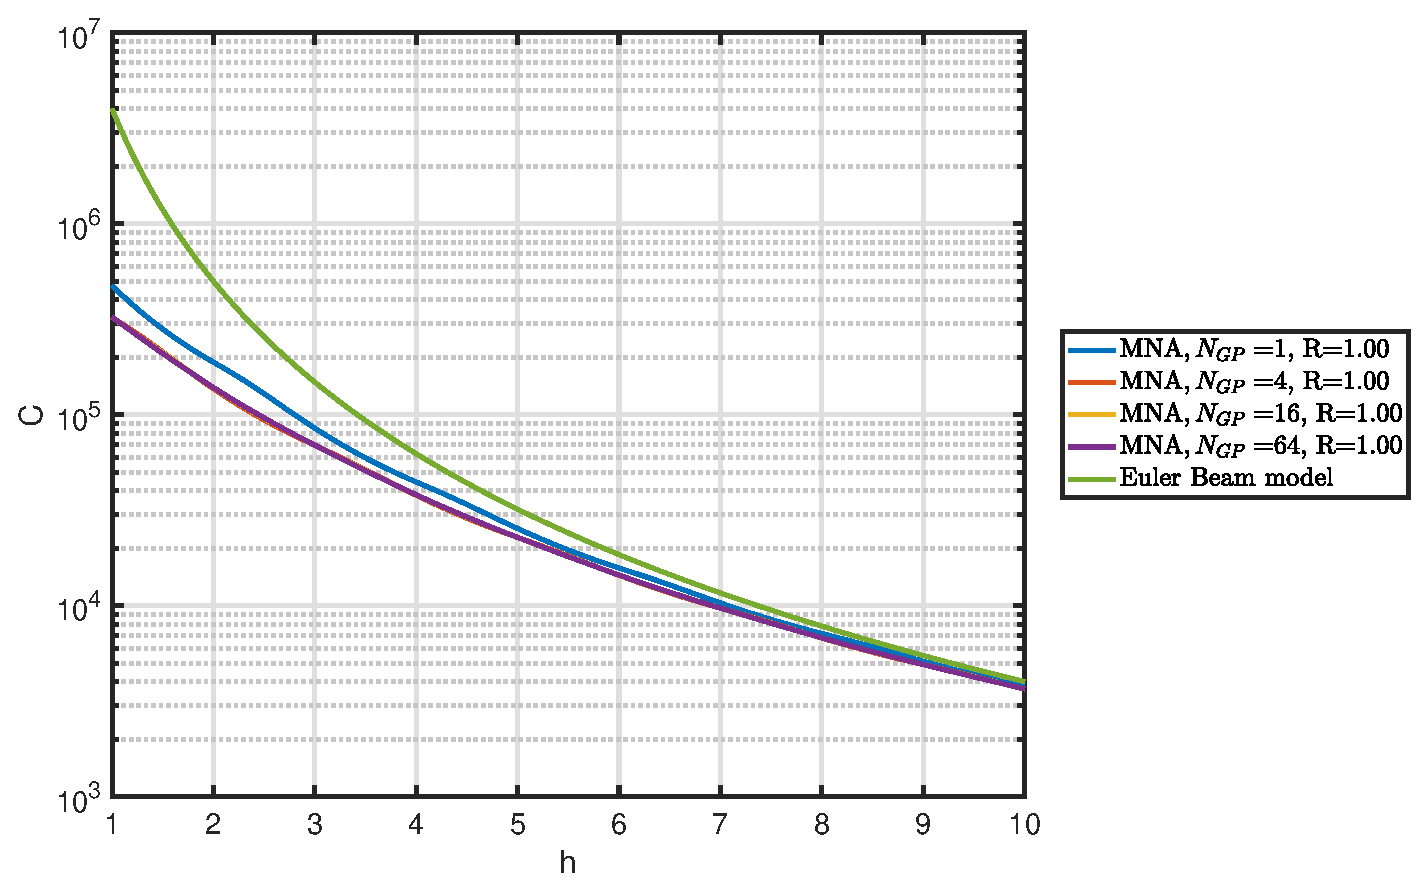
\includegraphics[width=0.4\textwidth]{images/Ch3/33e.eps} }}%
    \quad
    \subfloat[$h-V$ plot for $R=1$, $N_{GP}=\vecvar{1,4,16,64}$]{{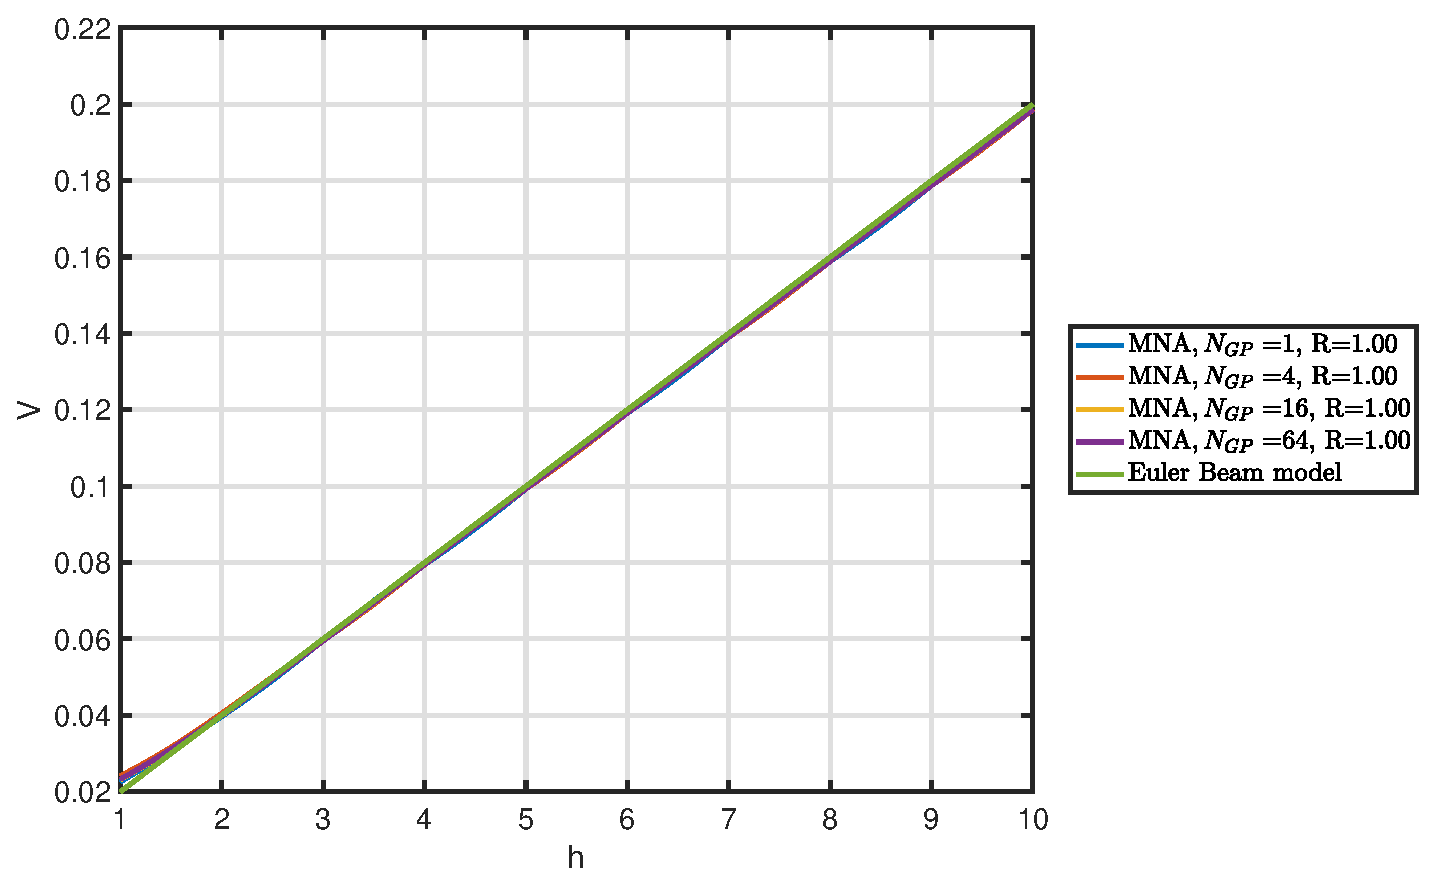
\includegraphics[width=0.4\textwidth]{images/Ch3/33f.eps}}}%
    \caption{Cantilever beam parametric study using the AMNA method. Effect of the sampling window size $R$ and of the number of Gauss points $N_{GP}$ on the structural compliance and the volume fraction. In each graph we reported in green the true theoretical values based on the analytic beam model.}%
    \label{fig:cbMNA}%
\end{figure*}
\clearpage
\section{MMA set-up}
\label{A1}
In this subsection we provide details of implementations considered for the method of moving asymptotes (MMA, \cite{svanberg1987method}). This approach makes local convex approximations at each iterations of both constraints and objective function. The convexity is adjusted by changing asymptotes' positions during the optimization history. A move limit can also be chosen in order to control the optimization step and avoid divergence. A correct scaling of both design variables and compliance is recommended to avoid numerical issues. Here we propose to re-scale variables and gradients according to:
\begin{eqnarray}
\hat{x}_j= \frac{x_j-l_{j}}{u_j-l_j}\\
\frac{dC}{d\hat{x}_j}=\frac{1}{u_j-l_j}\frac{dC}{dx_j}\\
\frac{dV}{d\hat{x}_j}=\frac{1}{u_j-l_j}\frac{dV}{dx_j}
\end{eqnarray}
where $l_j$ and $u_j$ are the $j^{th}$ - component respectively of the lower bound $\{l\}$ and of upper bound vector $\{u\}$. 
In order to avoid further MMA numerical issues one can either normalize the compliance dividing $C$ and $\vecvar{\frac{dC}{d\hat{x}}}$ by a constant $C_0$ greater than 1 that ensures the compliance and its gradient are small enough. However this way of normalizing introduces the issue of a good choice of $C_0$, depending on the particular problem studied. To avoid this problem, here we considered the following normalization:
\begin{eqnarray}
\hat{C}=\log{\left(1+C\right)}\\
\frac{d\hat{C}}{d\hat{x}_j}=\frac{1}{1+C}\frac{dC}{d\hat{x}_j}\\
\end{eqnarray}
Note that since $C>0$, $\log{\left(1+C\right)}$ is also greater than $0$. This ensures the gradients to be smaller for higher values of C (that is the case of ill connected configurations). In order to avoid MMA divergence due to uncontrolled optimization step length, here we propose a strategy that is similar to the one taken by the globally convergent version of MMA (GCMMA) \cite{svanberg2002class}. In the mmasub.m Matlab function called during the optimization loop we modified the updating of lowmin, lowmax, uppmin and uppmax formula, reducing the value of the coefficients that multiplies each variable range. This also means reducing the value set by default at 10 in equations \ref{eqnMNAl} and \ref{eqnMNAu}.
Accordingly this ensures the control of the optimization step through the overestimation of the problem convexity. In this way MMA behaves more conservatively at each iteration and is less prone to oscillate or to skip local optima\footnote{Note that this property can be beneficial or detrimental, depending on the case. Using classic MMA one can either skip worse local optima or better ones in the convergence history.}.